\documentclass[11pt,oneside]{article}    %use"amsart"insteadof"article"forAMSLaTeXformat
\usepackage{geometry}        %Seegeometry.pdftolearnthelayoutoptions.Therearelots.
\geometry{letterpaper}        %...ora4paperora5paperor...
%\geometry{landscape}        %Activateforforrotatedpagegeometry
%\usepackage[parfill]{parskip}        %Activatetobeginparagraphswithanemptylineratherthananindent
\usepackage{graphicx}                %Usepdf,png,jpg,orepsßwithpdflatex;useepsinDVImode
                                %TeXwillautomaticallyconverteps-->pdfinpdflatex        
\usepackage{amssymb}
\usepackage[colorlinks]{hyperref}

%----macros begin---------------------------------------------------------------
\usepackage{color}
\usepackage{amsthm}

\def\conv{\mbox{\textrm{conv}\,}}
\def\aff{\mbox{\textrm{aff}\,}}
\def\E{\mathbb{E}}
\def\R{\mathbb{R}}
\def\Z{\mathbb{Z}}
\def\tex{\TeX}
\def\latex{\LaTeX}
\def\v#1{{\bf #1}}
\def\p#1{{\bf #1}}
\def\T#1{{\bf #1}}

\def\vet#1{{\left(\begin{array}{cccccccccccccccccccc}#1\end{array}\right)}}
\def\mat#1{{\left(\begin{array}{cccccccccccccccccccc}#1\end{array}\right)}}

\def\lin{\mbox{\rm lin}\,}
\def\aff{\mbox{\rm aff}\,}
\def\pos{\mbox{\rm pos}\,}
\def\cone{\mbox{\rm cone}\,}
\def\conv{\mbox{\rm conv}\,}
\newcommand{\homog}[0]{\mbox{\rm homog}\,}
\newcommand{\relint}[0]{\mbox{\rm relint}\,}

%----macros end-----------------------------------------------------------------

\title{Hierarchical structures with LAR
\footnote{This document is part of the \emph{Linear Algebraic Representation with CoChains} (LAR-CC) framework~\cite{cclar-proj:2013:00}. \today}
}
\author{Alberto Paoluzzi}
%\date{}                            %Activatetodisplayagivendateornodate

\begin{document}
\maketitle
\nonstopmode

\tableofcontents



%===============================================================================
\section{Affine transformations}
%===============================================================================
%-------------------------------------------------------------------------------
\subsection{Design decision}
%-------------------------------------------------------------------------------
First we state the general rules that will be satisfied by the matrices used in this module, mainly devoted to apply affine transformations to vertices of models in structure environments:
\begin{enumerate}
\item assume the scipy \texttt{ndarray} as the type of vertices, stored in row-major order;
\item use the last coordinate as the homogeneous coordinate of vertices, but do not store it explicitly;
\item store explicitly the homogeneous coordinate of transformation matrices.
\item use labels '\texttt{verts}' and '\texttt{mat}' to distinguish between vertices and transformation matrices.
\item transformation matrices are dimension-independent, and their dimension is computed as the length of the parameter vector passed to the generating function.
\end{enumerate}


%-------------------------------------------------------------------------------
\subsection{Affine mapping}
%-------------------------------------------------------------------------------

%-------------------------------------------------------------------------------
@D Apply an affine transformation to a LAR model 
@{def larApply(affineMatrix):
    def larApply0(model):
        if isinstance(model,Model):
            # V = scipy.dot([v.tolist()+[1.0] for v in model.verts], affineMatrix.T).tolist()
            V = scipy.dot(array([v+[1.0] for v in model.verts]), affineMatrix.T).tolist()
            V = [v[:-1] for v in V]
            CV = copy.copy(model.cells)
            return Model((V,CV))
        elif isinstance(model,tuple) or isinstance(model,list):
            V,CV = model
            V = scipy.dot([v+[1.0] for v in V], affineMatrix.T).tolist()
            return [v[:-1] for v in V],CV
    return larApply0
@}
%-------------------------------------------------------------------------------


%-------------------------------------------------------------------------------
\subsection{Elementary matrices}
%-------------------------------------------------------------------------------
Elementary matrices for affine transformation of vectors in any dimensional vector space are defined here. They include translation, scaling, rotation and shearing. 

\paragraph{Translation}
%-------------------------------------------------------------------------------
@D Translation matrices
@{def t(*args): 
    d = len(args)
    mat = scipy.identity(d+1)
    for k in range(d): 
        mat[k,d] = args[k]
    return mat.view(Mat)
@}
%-------------------------------------------------------------------------------
\paragraph{Scaling}
%-------------------------------------------------------------------------------
@D Scaling matrices
@{def s(*args): 
    d = len(args)
    mat = scipy.identity(d+1)
    for k in range(d): 
        mat[k,k] = args[k]
    return mat.view(Mat)
@}
%-------------------------------------------------------------------------------
\paragraph{Rotation}
%-------------------------------------------------------------------------------
@D Rotation matrices
@{def r(*args): 
    args = list(args)
    n = len(args)
    @< plane rotation (in 2D) @>
    @< space rotation (in 3D) @>
    return mat.view(Mat)
@}
%-------------------------------------------------------------------------------
%-------------------------------------------------------------------------------
@D plane rotation (in 2D)
@{if n == 1: # rotation in 2D
    angle = args[0]; cos = COS(angle); sin = SIN(angle)
    mat = scipy.identity(3)
    mat[0,0] = cos;    mat[0,1] = -sin;
    mat[1,0] = sin;    mat[1,1] = cos;
@}
%-------------------------------------------------------------------------------
%-------------------------------------------------------------------------------
@D space rotation (in 3D)
@{if n == 3: # rotation in 3D
    mat = scipy.identity(4)
    angle = VECTNORM(args); axis = UNITVECT(args)
    cos = COS(angle); sin = SIN(angle)
    @< elementary rotations (in 3D) @>
    @< general rotations (in 3D) @>
@}
%-------------------------------------------------------------------------------
%-------------------------------------------------------------------------------
@D elementary rotations (in 3D)
@{if axis[1]==axis[2]==0.0:    # rotation about x
    mat[1,1] = cos;    mat[1,2] = -sin;
    mat[2,1] = sin;    mat[2,2] = cos;
elif axis[0]==axis[2]==0.0:    # rotation about y
    mat[0,0] = cos;    mat[0,2] = sin;
    mat[2,0] = -sin;    mat[2,2] = cos;
elif axis[0]==axis[1]==0.0:    # rotation about z
    mat[0,0] = cos;    mat[0,1] = -sin;
    mat[1,0] = sin;    mat[1,1] = cos;
@}
%-------------------------------------------------------------------------------
%-------------------------------------------------------------------------------
@D general rotations (in 3D)
@{else:        # general 3D rotation (Rodrigues' rotation formula)    
    I = scipy.identity(3) ; u = axis
    Ux = scipy.array([
        [0,        -u[2],      u[1]],
        [u[2],        0,     -u[0]],
        [-u[1],     u[0],         0]])
    UU = scipy.array([
        [u[0]*u[0],    u[0]*u[1],    u[0]*u[2]],
        [u[1]*u[0],    u[1]*u[1],    u[1]*u[2]],
        [u[2]*u[0],    u[2]*u[1],    u[2]*u[2]]])
    mat[:3,:3] = cos*I + sin*Ux + (1.0-cos)*UU
@}


%===============================================================================
\section{Structure types handling}
%===============================================================================

In order to implement a structure as a list of models and transformations, we need to be able to distinguish between two different types of scipy arrays. The first type is the one of arrays of vertices, the second one is the matrix array used to represent the fine transformations.

\subsection{\texttt{Mat} and \texttt{Verts} classes}
%-------------------------------------------------------------------------------
@D types Mat and Verts
@{""" class definitions for LAR """
import scipy
class Mat(scipy.ndarray): pass
class Verts(scipy.ndarray): pass
@}
%-------------------------------------------------------------------------------

\subsection{\texttt{Model} class}
%-------------------------------------------------------------------------------
@D Model class
@{class Model:
    """ A pair (geometry, topology) of the LAR package """
    def __init__(self,(verts,cells)):
        self.n = len(verts[0])
        # self.verts = scipy.array(verts).view(Verts)
        self.verts = verts
        self.cells = cells
    def __getitem__(self,i):
        return list((self.verts,self.cells))[i]
@}
%-------------------------------------------------------------------------------

\subsection{\texttt{Struct} iterable class}
%-------------------------------------------------------------------------------
@D Struct class
@{class Struct:
    """ The assembly type of the LAR package """
    def __init__(self,data,name='None'):
        self.body = data
        self.name = str(name)
        self.box = box(self) 
    def __name__(self):
        return self.name
    def __iter__(self):
        return iter(self.body)
    def __len__(self):
        return len(list(self.body))
    def __getitem__(self,i):
        return list(self.body)[i]
    def __print__(self): 
        return "<Struct name: %s>" % self.__name__()
    def __repr__(self):
        return "<Struct name: %s>" % self.__name__()
        #return "'Struct(%s,%s)'" % (str(self.body),str(str(self.__name__())))
@}
%-------------------------------------------------------------------------------


\subsection{\texttt{Struct} containment box}

%-------------------------------------------------------------------------------
@D Computation of the containment box of a Lar Struct or Model
@{""" Computation of the containment box of a Lar Struct or Model """
import copy
def box(model):
    if isinstance(model,Mat): return []
    elif isinstance(model,Struct):
        dummyModel = copy.deepcopy(model)
        dummyModel.body = [term if (not isinstance(term,Struct)) else [term.box,[[0,1]]]  for term in model.body]
        listOfModels = evalStruct( dummyModel )
        print "listOfModels =",listOfModels
        dim = len(listOfModels[0][0][0])
        theMin,theMax = box(listOfModels[0]) 
        for theModel in listOfModels[1:]:
            modelMin, modelMax = box(theModel)
            theMin = [val if val<theMin[k] else theMin[k] for k,val in enumerate(modelMin)]
            theMax = [val if val>theMax[k] else theMax[k] for k,val in enumerate(modelMax)]
        return [theMin,theMax]
    elif isinstance(model,Model):
        V = model.verts
    elif (isinstance(model,tuple) or isinstance(model,list)) and len(model)==2:
        V = model[0]
    coords = TRANS(V)
    theMin = [min(coord) for coord in coords]
    theMax = [max(coord) for coord in coords]
    return [theMin,theMax]
@}
%-------------------------------------------------------------------------------


%-------------------------------------------------------------------------------
\section{Structure to LAR conversion}
%-------------------------------------------------------------------------------


\subsection{Structure to pair (Vertices,Cells) conversion}
%-------------------------------------------------------------------------------
@D Structure to pair (Vertices,Cells) conversion
@{""" Structure to pair (Vertices,Cells) conversion """

def struct2lar(structure):
    listOfModels = evalStruct(structure)
    vertDict = dict()
    index,defaultValue,CW,W = -1,-1,[],[]
        
    for model in listOfModels:
        if isinstance(model,Model):
            V,FV = model.verts,model.cells
        elif (isinstance(model,tuple) or isinstance(model,list)) and len(model)==2:
            V,FV = model
        for k,incell in enumerate(FV):
            outcell = []
            for v in incell:
                key = vcode(V[v])
                if vertDict.get(key,defaultValue) == defaultValue:
                    index += 1
                    vertDict[key] = index
                    outcell += [index]
                    W += [eval(key)]
                else: 
                    outcell += [vertDict[key]]
            CW += [outcell]
            
    return W,CW
@}
%-------------------------------------------------------------------------------
\subsection{Embedding or projecting LAR models}
%-------------------------------------------------------------------------------

In order to apply 3D transformations to a two-dimensional LAR model, we must embed it in 3D space, by adding one more coordinate to its vertices. 

\paragraph{Embedding or projecting a geometric model}

This task is performed by the function \texttt{larEmbed} with parameter $k$, that inserts its $d$-dimensional geometric argument in the $x_{d+1}, \ldots, x_{d+k}=0$ subspace of $\E^{d+k}$.
A projection transformation, that removes the last $k$ coordinate of vertices, without changing the object topology, is performed by the function \texttt{larEmbed} with \emph{negative} integer parameter.


%-------------------------------------------------------------------------------
@D Embedding and projecting a geometric model
@{def larEmbed(k):
    def larEmbed0(model):
        V,CV = model
        if k>0:
            V = [v+[0.]*k for v in V] 
        elif k<0:
            V = [v[:-k] for v in V] 
        return V,CV
    return larEmbed0
@}
%-------------------------------------------------------------------------------

%===============================================================================
\section{Hierarchical complexes}
%===============================================================================
Hierarchical models of complex assemblies are generated by an aggregation
of subassemblies, each one defined in a local coordinate system, and
relocated by affine transformations of coordinates.  This operation
may be repeated hierarchically, with some subassemblies defined by
aggregation of simpler parts, and so on, until one obtains a set of
elementary components, which cannot be further decomposed.

Two main advantages can be found in a hierarchical modeling approach. Each elementary part and each assembly, at every hierarchical level, are defined independently from each other, using a local coordinate frame, suitably chosen to make its definition easier. Furthermore, only one copy of each component is stored in the memory, and may be instanced in different locations and orientations how many times it is needed.

%-------------------------------------------------------------------------------
\subsection{Traversal of hierarchical structures}
%-------------------------------------------------------------------------------

Of course, the main algorithm with hierarchical structures is the \emph{traversal} of the structure network, whose aim is to transform every encountered object from local to global coordinates, where the global coordinates are those of the network root (the only node with indegree zero).

A structure network can be modelled using a directed acyclic multigraph, i.e.~a triple $(N,A,f)$
made by a set $N$ of nodes, a set $A$ of arcs, and a function $f:A \to N^2$ from arcs to ordered pairs of nodes. Conversely that in standard oriented graphs, in this kind of structure more than one oriented arc is allowed between the same pair on nodes.

\begin{figure}[htbp] %  figure placement: here, top, bottom, or page
   \centering
   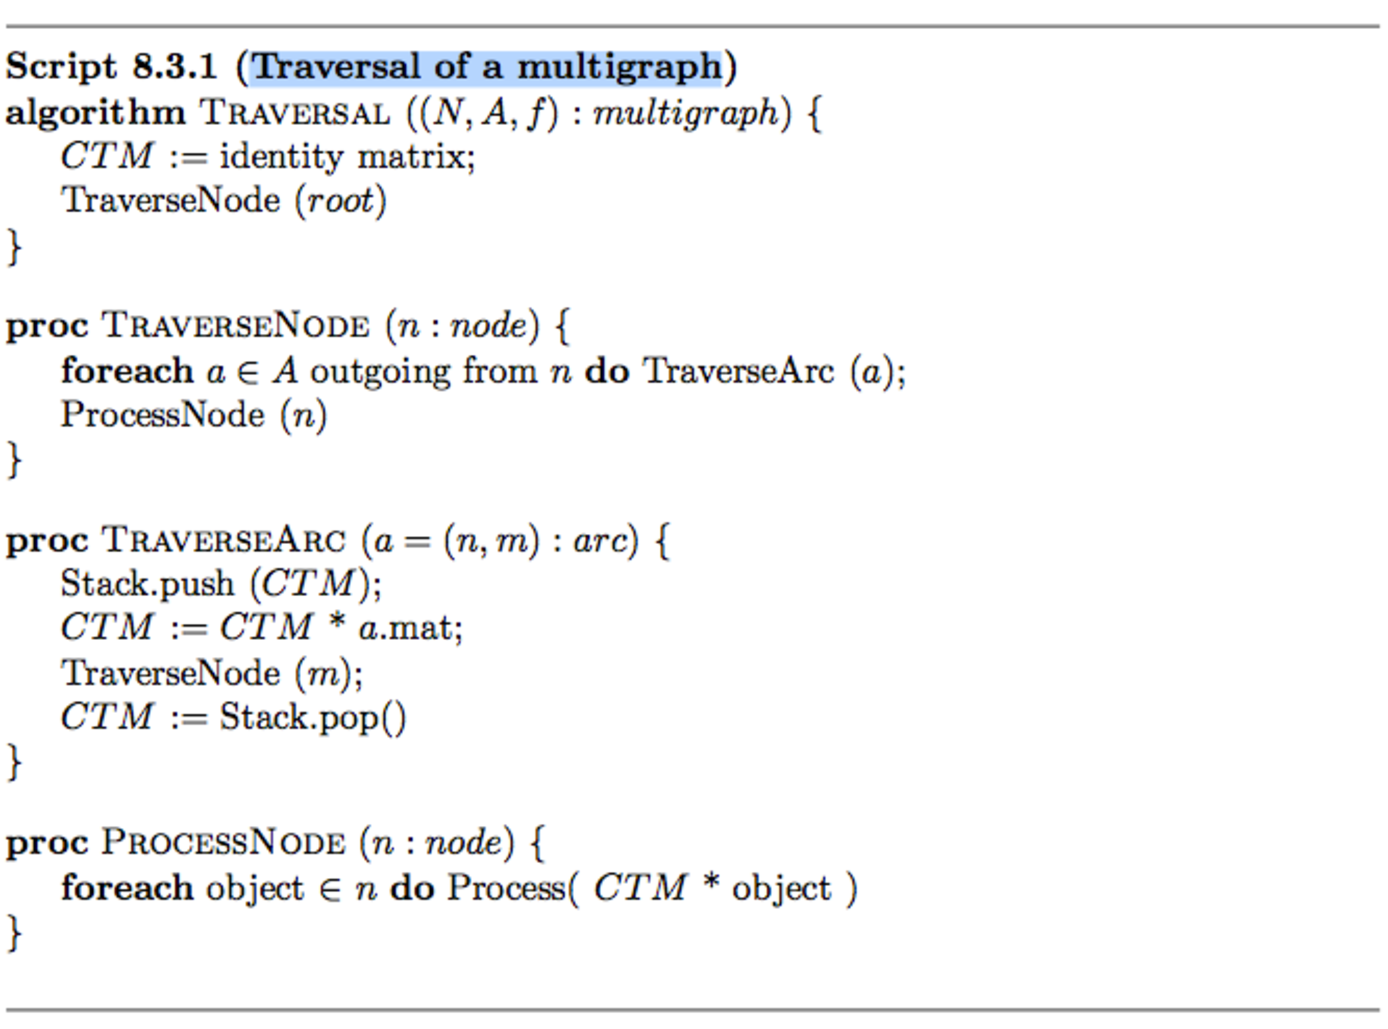
\includegraphics[width=0.8\linewidth]{images/traversal} 
   \caption{Traversal algorithm of an acyclic multigraph.}
   \label{fig:traversal}
\end{figure}

A simple modification of a DFS (Depth First Search) visit of a graph can be used to traverse the structure network This algorithm is given in Figure~\ref{fig:traversal} from~\cite{Paoluzzi2003a}. 

\subsubsection{Traversal of nested lists}

The representation chosen for structure networks with LAR is the serialised one, consisting in ordered sequences (lists) of either (a) LAR models, or (b) affine transformations, or (c) references to other structures, either directly nested within some given structure, or called by reference (name) from within the list.

The aim of a structure network traversal is, of course, to transform every component structure, usually defined in a local coordinate system, into the reference frame of the structure as a whole, normally corresponding with the reference system of the structure's root, called the \emph{world coordinate} system.

\paragraph{The pattern of calls and returned values}

In order to better understand the behaviour of the traversal algorithm, where every transformation is applied to all the following models, --- but only if included in the same structure  (i.e.~list) --- it may be very useful to start with an \emph{algorithm emulation}. In particular, the recursive script below discriminates between three different cases (number, string, or sequence), whereas the actual traversal must do with (a) Models, (b) Matrices, and (c) Structures, respectively.

%-------------------------------------------------------------------------------
@D Emulation of scene multigraph traversal
@{from pyplasm import *
def __traverse(CTM, stack, o):
    for i in range(len(o)):
        if ISNUM(o[i]): print o[i], REVERSE(CTM)
        elif ISSTRING(o[i]): 
            CTM.append(o[i])
        elif ISSEQ(o[i]):
            stack.append(o[i])                # push the stack
            __traverse(CTM, stack, o[i])
            CTM = CTM[:-len(stack)]         # pop the stack

def algorithm(data):
    CTM,stack = ["I"],[]
    __traverse(CTM, stack, data)  
@}
%-------------------------------------------------------------------------------

Some use example of the above algorithm are provided below. The printout produced at run time is shown from the \texttt{emulation of traversal algorithm} macro.
%-------------------------------------------------------------------------------
@D Examples of multigraph traversal
@{data = [1,"A", 2, 3, "B", [4, "C", 5], [6,"D", "E", 7, 8], 9]  
print algorithm(data)
>>> 1 ['I']
    2 ['A', 'I']
    3 ['A', 'I']
    4 ['B', 'A', 'I']
    5 ['C', 'B', 'A', 'I']
    6 ['B', 'A', 'I']
    7 ['E', 'D', 'B', 'A', 'I']
    8 ['E', 'D', 'B', 'A', 'I']
    9 ['B', 'A', 'I']

data = [1,"A", [2, 3, "B", 4, "C", 5, 6,"D"], "E", 7, 8, 9]  
print algorithm(data)
>>> 1 ['I']
    2 ['A', 'I']
    3 ['A', 'I']
    4 ['B', 'A', 'I']
    5 ['C', 'B', 'A', 'I']
    6 ['C', 'B', 'A', 'I']
    7 ['E', 'A', 'I']
    8 ['E', 'A', 'I']
    9 ['E', 'A', 'I']
@}
%-------------------------------------------------------------------------------
%-------------------------------------------------------------------------------
@D Emulation of traversal algorithm
@{dat = [2, 3, "B", 4, "C", 5, 6,"D"]
print algorithm(dat)
>>> 2 ['I']
    3 ['I']
    4 ['B', 'I']
    5 ['C', 'B', 'I']
    6 ['C', 'B', 'I']
data = [1,"A", dat, "E", 7, 8, 9]
print algorithm(data)
>>> 1 ['I']
    2 ['A', 'I']
    3 ['A', 'I']
    4 ['B', 'A', 'I']
    5 ['C', 'B', 'A', 'I']
    6 ['C', 'B', 'A', 'I']
    7 ['E', 'A', 'I']
    8 ['E', 'A', 'I']
    9 ['E', 'A', 'I']
@}
%-------------------------------------------------------------------------------

\paragraph{Traversal of a scene multigraph}

The previous traversal algorithm is here customised for scene multigraph, where the objects are LAR models, i.e.~pairs of vertices of type '\texttt{Verts} and cells, and where the transformations are matrix transformations of type '\texttt{Mat}'.

\paragraph{Check models for common dimension}
The input list of a call to \texttt{larStruct} primitive is preliminary checked for uniform dimensionality of the enclosed LAR models and transformations. The common dimension \texttt{dim} of models and matrices is returned by the function \texttt{checkStruct}, within the class definition \texttt{Struct} in the module \texttt{lar2psm}. Otherwise, an exception is generated (TODO).


%-------------------------------------------------------------------------------
@D Check for dimension of a structure element (Verts or V)
@{@< Flatten a list @>
def checkStruct(lst):
    """ Return the common dimension of structure elements.

        TODO: aggiungere test sulla dimensione minima delle celle (legata a quella di immersione)
    """
    print "lst =",lst
    print "flatten(lst) =",flatten(lst)
    vertsDims = [computeDim(obj) for obj in flatten(lst)]
    vertsDims = [dim for dim in vertsDims if dim!=None and dim!=0]
    if EQ(vertsDims) and len(vertsDims)!=0: 
        return vertsDims[0]
    else: 
        print "\n vertsDims =", vertsDims
        print "*** LAR ERROR: Struct dimension mismatch."

def computeDim(obj):
    """ Check for dimension of a structure element (Verts or V). 
    """
    if (isinstance(obj,Model)):
        return obj.n
    elif (isinstance(obj,tuple) or isinstance(obj,list)) and len(obj)==2:
        V = obj[0]
        if (isinstance(V,list) and isinstance(V[0],list) and 
                (isinstance(V[0][0],float) or isinstance(V[0][0],int))): 
            dim = len(V[0])
            return dim
    elif (isinstance(obj,Mat)):
        dim = obj.shape[0]-1
        return dim
    else: return 0
@}
%-------------------------------------------------------------------------------

\paragraph{Flatten a list using Python generators}
The \texttt{flatten} is a generator that yields the non-list values of its input in order. In the example, the generator is converted back to a list before printing. Modified from \href{http://rosettacode.org/wiki/Flatten_a_list#Python}{\emph{Rosetta code}} project. It is used here to flatten a structure in order to check for common dimensionality of elements.

%-------------------------------------------------------------------------------
@D Flatten a list
@{""" Flatten a list using Python generators """
def flatten(lst):
    for x in lst:
        if (isinstance(x,tuple) or isinstance(x,list)) and len(x)==2:
            yield x
        elif (isinstance(x,tuple) or isinstance(x,list)):
            for x in flatten(x):
                yield x
        elif isinstance(x, Struct):
            for x in flatten(x.body):
                yield x
        else:
            yield x
 
#  lst = [[1], 2, [[3,4], 5], [[[]]], [[[6]]], 7, 8, []]
#  print list(flatten(lst)) 
#  [1, 2, 3, 4, 5, 6, 7, 8]

#  import itertools
#  chain = itertools.chain.from_iterable([[1,2],[3],[5,89],[],[6]])
#  print(list(chain))
#  [1, 2, 3, 5, 89, 6]    ###  TODO: Bug coi dati sopra?
@}
%-------------------------------------------------------------------------------

\paragraph{Initialization and call of the algorithm}

The function \texttt{evalStruct} is used to evaluate a structure network, i.e.~to return a \texttt{scene}
list of objects of type \texttt{Model}, all referenced in the world coordinate system. The input variable \texttt{struct} must contain an object of class \texttt{Struct}, i.e.~a reference to an unevaluated structure network. The variable \texttt{dim}  contains the embedding dimension of the structure, i.e.~the number of doordinates of its vertices (normally either 2 or 3), the CTM (Current Transformation Matrix) is initialised to the (homogeneous) identity matrix, and  the \texttt{scene} is returned by calling the \texttt{traverse} algorithm.

%-------------------------------------------------------------------------------
@D Traversal of a scene multigraph
@{""" Traversal of a scene multigraph """
@< Structure traversal algorithm @>
def evalStruct(struct):
    dim = checkStruct(struct.body)
    print "\n dim =",dim
    CTM, stack = scipy.identity(dim+1), []
    print "\n CTM, stack =",CTM, stack
    scene = traversal(CTM, stack, struct, []) 
    return scene
@}
%-------------------------------------------------------------------------------

\paragraph{Structure traversal algorithm}

The \texttt{traversal} algorithm decides between three different cases, depending on the type of the currently inspected object. If the object is a \texttt{Model} instance, then applies to it the \texttt{CTM} matrix; else if the object is a \texttt{Mat} instance, then the \texttt{CTM} matrix is updated by (right) product with it; else if the object is a \texttt{Struct} instance, then the \texttt{CTM} is pushed on the stack, initially empty, then the \texttt{traversal} is called (recursion), and finally, at (each) return from recursion, the \texttt{CTM} is recovered by popping the stack.

%-------------------------------------------------------------------------------
@D Structure traversal algorithm 
@{def traversal(CTM, stack, obj, scene=[]):
    print "\n CTM, obj =",obj
    for i in range(len(obj)):
        if isinstance(obj[i],Model): 
            scene += [larApply(CTM)(obj[i])]
        elif (isinstance(obj[i],tuple) or isinstance(obj[i],list)) and len(obj[i])==2:
            scene += [larApply(CTM)(obj[i])]
        elif isinstance(obj[i],Mat): 
            CTM = scipy.dot(CTM, obj[i])
        elif isinstance(obj[i],Struct):
            stack.append(CTM) 
            traversal(CTM, stack, obj[i], scene)
            CTM = stack.pop()
    return scene
@}
%-------------------------------------------------------------------------------


%===============================================================================
\section{Larstruct exporting}
%===============================================================================
\label{sec:larstruct}
Here we assemble top-down the \texttt{lar2psm} module, by orderly listing the functional parts it is composed of. Of course, this one is the module version corresponding to the current state of the system, i.e.~to a very initial state. Other functions will be added when needed.
%------------------------------------------------------------------
@O lib/py/larstruct.py
@{"""Module with functions needed to interface LAR with pyplasm"""
@< Function to import a generic module @>
from lar2psm import *
@< Translation matrices @>
@< Scaling matrices @>
@< Rotation matrices @>
@< Embedding and projecting a geometric model @>
@< Apply an affine transformation to a LAR model @>
@< Check for dimension of a structure element (Verts or V) @>
@< Traversal of a scene multigraph @>
@< types Mat and Verts @>
@< Model class @>
@< Struct class @>
@< Structure to pair (Vertices,Cells) conversion @>
@< Embedding and projecting a geometric model @>
@< Computation of the containment box of a Lar Struct or Model @>
@}
%------------------------------------------------------------------

%-------------------------------------------------------------------------------
%===============================================================================
\section{Examples}
%===============================================================================
%-------------------------------------------------------------------------------
Some examples of structures as combinations of LAR models and affine transformations are given in this section. 

\paragraph{Global coordinates}
We start with a simple 2D example of a non-nested list of translated 2D object instances and rotation about the origin.

%-------------------------------------------------------------------------------
@O test/py/larstruct/test04.py
@{""" Example of non-nested structure with translation and rotations """
import sys; sys.path.insert(0, 'lib/py/')
from largrid import *
from larstruct import *
square = larCuboids([1,1])
table = larApply( t(-.5,-.5) )(square)
chair = larApply( s(.35,.35) )(table)
chair1 = larApply( t(.75, 0) )(chair)
chair2 = larApply( r(PI/2) )(chair1)
chair3 = larApply( r(PI/2) )(chair2)
chair4 = larApply( r(PI/2) )(chair3)
VIEW(SKEL_1(STRUCT(MKPOLS(table)+MKPOLS(chair1)+
                   MKPOLS(chair2)+MKPOLS(chair3)+MKPOLS(chair4))))
@}
%-------------------------------------------------------------------------------

\paragraph{Local coordinates}
A different composition of transformations, from local to global coordinate frames, is used in the following example.

%-------------------------------------------------------------------------------
@O test/py/larstruct/test05.py
@{""" Example of non-nested structure with translation and rotations """
import sys; sys.path.insert(0, 'lib/py/')
from largrid import *
from larstruct import *
square = larCuboids([1,1])
square = Model(square)
table = larApply( t(-.5,-.5) )(square)
chair = larApply( s(.35,.35) )(table)
chair = larApply( t(.75, 0) )(chair)
struct = Struct([table] + 4*[chair, r(PI/2)])
scene = evalStruct(struct)
VIEW(SKEL_1(STRUCT(CAT(AA(MKPOLS)(scene)))))
@}
%-------------------------------------------------------------------------------

\paragraph{Call of nested structures by reference}
Finally, a similar 2D example is given, by nesting one (or more) structures via separate definition and call by reference from the interior. Of course, a cyclic set of calls must be avoided, since it would result in a \emph{non acyclic} multigraph of the structure network.

%-------------------------------------------------------------------------------
@O test/py/larstruct/test06.py
@{""" Example of nested structures with translation and rotations """
import sys; sys.path.insert(0, 'lib/py/')
from largrid import *
from larstruct import *
square = larCuboids([1,1])
square = Model(square)
table = larApply( t(-.5,-.5) )(square)
chair = Struct([ t(.75, 0), s(.35,.35), table ])
struct = Struct( [t(2,1)] + [table] + 4*[r(PI/2), chair])
struct = Struct(10*[struct,t(0,2.5)])
struct = Struct(10*[struct,t(3,0)])
scene = evalStruct(struct)
VIEW(SKEL_1(STRUCT(CAT(AA(MKPOLS)(scene)))))
@}
%-------------------------------------------------------------------------------


%-------------------------------------------------------------------------------
@O test/py/larstruct/test08.py
@{""" LAR model input and handling """
@< Input of LAR architectural plan @>
dwelling = larApply(t(3,0))(Model((V,FV)))
print "\n dwelling =",dwelling
VIEW(EXPLODE(1.2,1.2,1)(MKPOLS(dwelling)))
plan = Struct([dwelling,s(-1,1),dwelling])
VIEW(EXPLODE(1.2,1.2,1)(CAT(AA(MKPOLS)(evalStruct(plan)))))
@}
%-------------------------------------------------------------------------------



%-------------------------------------------------------------------------------
@D Input of LAR architectural plan
@{@< Initial import of modules @>
from mapper import *
V = [[3,-3],
[9,-3],[0,0],[3,0],[9,0],[15,0],
[3,3],[6,3],[9,3],[15,3],[21,3], 
[0,9],[6,9],[15,9],[18,9],[0,13],
[6,13],[9,13],[15,13],[18,10],[21,10], 
[18,13],[6,16],[9,16],[9,17],[15,17],
[18,17],[-3,24],[6,24],[15,24],[-3,13]]
FV = [
[22,23,24,25,29,28], [15,16,22,28,27,30], [18,21,26,25], 
[13,14,19,21,18], [16,17,23,22], [11,12,16,15],
[9,10,20,19,14,13], [2,3,6,7,12,11], [0,1,4,8,7,6,3],
[4,5,9,13,18,17,16,12,7,8],[17,18,25,24,23]]
@}
%-------------------------------------------------------------------------------



\paragraph{Transformation of Struct object to LAR model pair}

The following test application first generates a grid $3\times 3$ of LAR cubes, extracts
its boundary cells as \texttt{BV}, then produces a \texttt{struct} object with 30 translated instances of it,
and finally transforms the \texttt{struct} object into a LAR pair \texttt{W,FW}.
Let us notice that due to the assembly process, some 2-cells in \texttt{FW} are doubled.

%-------------------------------------------------------------------------------
@O test/py/larstruct/test09.py
@{""" Transformation of Struct object to LAR model pair """
import sys
""" import modules from larcc/lib """
sys.path.insert(0, 'lib/py/')
from larstruct import *

@< Transform Struct object to LAR model pair @>
@}
%-------------------------------------------------------------------------------

The actual generation of the structure and its transformation to a LAR model pair is actually performed in the following macro.

%-------------------------------------------------------------------------------
@D Transform Struct object to LAR model pair
@{""" Generation of Struct object and transform to LAR model pair """
cubes = larCuboids([10,10,10],True)
V = cubes[0]
FV = cubes[1][-2]
CV = cubes[1][-1]
bcells = boundaryCells(CV,FV)
BV = [FV[f] for f in bcells]
VIEW(EXPLODE(1.2,1.2,1.2)(MKPOLS((V,BV))))

block = Model((V,BV))
struct = Struct(10*[block, t(10,0,0)])
struct = Struct(10*[struct, t(0,10,0)])
struct = Struct(3*[struct, t(0,0,10)])
W,FW = struct2lar(struct)

VIEW(EXPLODE(1.2,1.2,1.2)(MKPOLS((W,FW))))
@}
%-------------------------------------------------------------------------------



%===============================================================================
\appendix
%===============================================================================
\subsection{Importing a generic module}
First we define a parametric macro to allow the importing of \texttt{larcc} modules from the project repository \texttt{lib/py/}. When the user needs to import some project's module, she may call this macro as done in Section~\ref{sec:lar2psm}.
%------------------------------------------------------------------
@d Import the module
@{import sys; sys.path.insert(0, 'lib/py/')
import @1
@}
%------------------------------------------------------------------

\paragraph{Importing a module} A function used to import a generic \texttt{lacccc} module within the current environment is also useful.
%------------------------------------------------------------------
@d Function to import a generic module
@{def importModule(moduleName):
    @< Import the module @(moduleName@) @>
@| importModule @}
%------------------------------------------------------------------



\bibliographystyle{amsalpha}
\bibliography{larstruct}

\end{document}
